\par Бурное развитие средств вычислительной техники в последнее десятилетие дало новый толчок развитию стеганографии. В отличие от криптографии, которая скрывает содержимое секретного сообщения, стеганография скрывает сам факт его существования. Стеганографию обычно используют совместно с методами криптографии, таким образом, дополняя её. 
\par Для защиты авторских прав мультимедийных файлов применяется создание и внедрение цифровых водяных знаков (ЦВЗ). ЦВЗ отличаются от криптографической ЭЦП тем, что информация «встроена» прямо в сигнал. Стеганографические цифровые водяные знаки невидимы, благодаря этому удается сохранить в тайне сам факт наличия метки, что служит дополнительным фактором защиты. 

\par Процесс формирования водяного знака может быть описан следующим образом. Сначала в сигнал-источник $S$ в доверенной среде внедряются водяные знаки при помощи функции $E$. В результате получается сигнал $S_E$. Следующий этап — распространение $S_E$ через сеть или любым другим способом. Во время распространения на сигнал может быть совершена атака. 
У получившегося сигнала $S_{EA}$ водяные знаки могут быть потенциально уничтожены или изменены. На следующем этапе функция обнаружения $D$ пытается обнаружить водяные знаки $\omega$. Отсутствие или повреждение водяного знака свидетельствует о подмене оригинального сигнала. А наличие неизменного знака $\omega$, подтверждает целостность полученных данных. Весь жизненный цикл цифрового водяного знака представлен на рисунке \ref{fig:DWMLifiCircle}.
\begin{figure}[h]
\centering
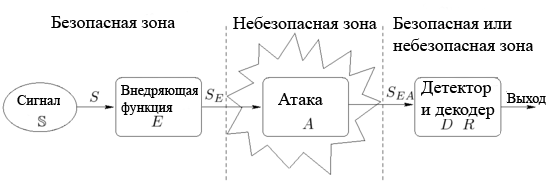
\includegraphics[width=0.9\linewidth]{./DWMLifiCircle}
\caption[Цикл стеганографической ЭЦП]{Цикл стеганографической ЭЦП \cite{lu2004}}
\label{fig:DWMLifiCircle}
\end{figure}

\par В работе \cite{gupta2015} представлена классификация ЦВЗ и подробный обзор методов их встраивания в исходные данные. Так по надежности выделяют следующие группы водяных знаков:
\begin{itemize}
\item \textit{чрупкие} -- нечитаемые, при малейшей модификации данных;
\item \textit{полу-хрупкие} -- выдерживаю незначительные изменения данных, но при вредоносном изменении становятся нечитаемыми, подобно хрупким;
\item \textit{надёжные}  -- противостоящие всем известным видам атак.
\end{itemize}
\par Методы нанесения ЦВЗ делятся на пространственные и частотные. 

 К пространственным методам относится метод \textit{LSB (Least Significant Bit)}.
Суть этого метода заключается в замене последних значащих битов в контейнере
 (изображения, аудио или видеозаписи) на биты скрываемого сообщения. Разница между пустым и заполненным контейнерами должна быть не ощутима
  для органов восприятия человека. Методы LSB являются неустойчивыми ко всем видам атак и могут быть использованы только при отсутствии шума в канале передачи данных.

Пример частотного метода нанесения ЦВЗ -- метод расширения спектра. Метод амплитудной модуляции, схожий с методом расширения спектра, также применяется для внедрения. Метод квантования не очень надёжен, но позволяет внедрить большой объём информации.
 Данные методы основываются на применении инвертируемых преобразованиях, таких как дискретное преобразование вейвлет или фурье, к несущему контейнеру. Добавление водяного знака осуществляется модификацией коэффициентов разложения (спектра) в соответствии с выбранным алгоритмом внедрения ЦВЗ. В завершении, применяется обратное преобразование для получение контейнера, содержащего ЦВЗ. Данные методы неравномерно распределяют встраиваемую информацию в несущий контейнер, делая задачу обнаружения и манипулирования с ЦВЗ сравнительно сложнее, по сравнению с пространственными методами встраивания. ЦВЗ, как правило, встраивается в средние частоты исходного сигнала, так как высокие частоты легко разрушаются операциями сжатия или масштабирвоания, а низкие частоты содержат основную воспринимаемую человеком информацию \cite{asatryan2009}. Это делает ЦВЗ, встроенный этими методами надежным или
  отличаются средней надёжностью, но очень маленьким информационной
   ёмкостью. 
   
   \par И частотные и пространственные методы имеют свои недостатки и особенности. Так недостатком частотных методов, может считаться высокая вычислительная сложность алгоритмов и малый объем встраиваемой информации, а пространственных относительная легкость обнаружения и ненадежностью. Поэтому в последнее время все больше внимание уделяется гибридизации данных методов, с целью получить заданные характеристики алгоритма встраивания и извлечения ЦВЗ. Так в работе \cite{deguillaume2003} исследователи представили гибридный метод, объединяющий свойства надежных и хрупких ЦВЗ. Надежный и хрупкий водяные знаки встраиваются в исходный сигнал последовательно. В работе \cite{al2007} исследователи поставили задачу улучшения производительности существующих методов. Для этого они разработали комбинированный подход на основе ДВП (дискретные вейвлет-преобразования) и ДКП (дискретное косинусное преобразование). В соответствии с данным подходом встраивание происходит на основе ДКП в двухуровневое ДВП от исходного сигнала (рисунок \ref{fig:HybridWM}).
   \begin{figure}[h]
\centering
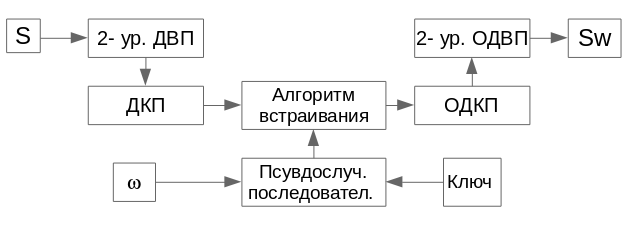
\includegraphics[width=0.7\linewidth]{./HybridWM}
\caption{Комбинирвоанная процедура формирования ЦВЗ.}
\label{fig:HybridWM}
\end{figure}

   



